
%(BEGIN_QUESTION)
% Copyright 2008, Tony R. Kuphaldt, released under the Creative Commons Attribution License (v 1.0)
% This means you may do almost anything with this work of mine, so long as you give me proper credit

A chlorine analyzer measures the chlorine concentration in wastewater, to determine whether or not there is sufficient chlorine dissolved in the wastewater to properly disinfect it prior to discharging into a natural body of water such as a river or bay:

$$\includegraphics[width=15.5cm]{i00679x01.eps}$$

There is a problem with this system, though: the valves and hoses inside the chlorine analyzer keep bursting because the sample pressure is too great.  The analyzer is designed for a maximum sample water pressure of 1 PSI, and the pipe is pressurized to 10 PSI.

\filbreak

An instrument technician figures out a solution to this dilemma.  His solution involves installing an open-top ``standpipe'' where water from the main wastewater pipe enters before flowing into the analyzer:

$$\includegraphics[width=15.5cm]{i00679x02.eps}$$

Describe how the technician's solution avoids the overpressure problem.

\underbar{file i00679}
%(END_QUESTION)





%(BEGIN_ANSWER)

With the standpipe installed, wastewater flows to the analyzer by gravity (hydrostatic pressure) alone.  The main wastewater pipe pressure is completely isolated from the analyzer.

%(END_ANSWER)





%(BEGIN_NOTES)

This problem was encountered and solved by a former student (Bryce VanWerven) at his workplace in a municipal wastewater treatment plant.  The standpipe solution is his idea and not mine!

%INDEX% Measurement, analytical: chlorine in water
%INDEX% Physics, static fluids: hydrostatic pressure

%(END_NOTES)


